\documentclass[11pt]{article}

\usepackage{amsmath,amssymb,amsfonts}
\usepackage{mathtools}
\usepackage{graphicx}
\usepackage{tikz}
\usepackage{xcolor}
\usepackage{soul}
\usepackage{hyperref}
\hypersetup{
	colorlinks=true,
	linkcolor=blue,
	filecolor=magenta,      
	urlcolor=cyan,
	pdftitle={Overleaf Example},
	pdfpagemode=FullScreen,
}
\newcommand{\redcircle}[1]{%
	\tikz[baseline=(char.base)]{
		\node[shape=circle, draw=red, text=red, thick, inner sep=1pt] (char) {\textbf{#1}};
	}%
}
\setul{1pt}{3pt} % Linienhöhe und Abstand zum Text (optional anpassbar)

\setlength{\topmargin}{-.5in} \setlength{\textheight}{9.25in}
\setlength{\oddsidemargin}{0in} \setlength{\textwidth}{6.8in}
\setlength{\parindent}{0pt}

\begin{document}
	
	\Large
	
	
	\noindent{\bf Teil 1: Differentialgleichung im $\mathbb{R}$}
	
	
	
	\medskip\hrule\medskip
	\underline{an1: Der $\mathbb{R}^n$ als normierter Vektorraum}\\
	\underline{Stichworte}: $\mathbb{R}^n$ mit Normen $||\cdot||_{\infty}, ||\cdot||_2$, (Folgen)Konvergenz , GWSätze, Projektionen\\
	\medskip\hrule\medskip
	\underline{Literatur: [Hoff], Kapitel 9.1}\\
	Hier und im gesamten Skript steht [Hoff] für das Buch\\
	\underline{Dieter Hoffmann: Analysis für Wirtschaftswissenschaftler und Ingenieure},\\
	Siehe auch die Literaturangaben auf der Website der Vorlesung zur \href{https://www.math.uni-duesseldorf.de/~internet/Ana2_SoSe25/#veranstaltungen}{Analysis II}\\
	in diesem Buch finden Sie bestimmte Skript teile ausführlicher aufgeschrieben.\\
	\medskip\hrule\medskip
	\textbf{1.1. \underline{Bedingungsanleitung}} der Vorlesung "Analysis II" 
	(wie schon in "Analysis I"):\\
	-vor jedem Termin erscheint auf der Website Kurzfristig ein neues 
	Kurz-Skriptteil zur nächsten Vorlesungssitzung. Sie können einen 
	Vorab-Blick hineinwerfen.\\
	-Besuchen Die unbedingt die Vorlesungstermine! Das Skript wird dort ausführlich erklärt, erläutert , entwickelt und veranschaulicht. Der Stoff ist ohne den zugehörigen mündlichen Ergänzungen nicht zu erfassen.\\
	-Lesen die zusätzlich ergänzende \underline{Literatur} im Selbststudium, 
	etwa die angegebene Literatur, was gier Häufig das Buch [Hoff] ist.\\
	Überlegen Sie selbstständig die angegebenen Übungsvorschläge, die mit dem Übungssmiley \redcircle{Ü} markiert sind. Sprechen Sie mit anderen darüber.\\
	-Besuchen Die regelmäßig das Tutorium/Ihre Übungsgruppe, um weitere 
	Beispiele Kennenzulernen und fleißig zu üben.
	-Das Skript enthält einen Farbcode: \setulcolor{yellow}\ul{Gelb} für Notationen/Bezeichnungen,\\
	\setulcolor{red}\ul{rot unterstrichen} werden Begriffdefinitionen und Namen wichtiger Sätze,\\
	\setulcolor{blue}\ul{blau unterstrichen} werden Referenznummern und Zitierungen,\\
	\setulcolor{green}\ul{grün unterstrichen} werden 
	Behauptungen/Sätze/Lemmas/Korollare,\\
	\setulcolor{orange}\ul{orange unterstrichen} werden wesentliche Beweisideen.\\
	In Analysis II geht es in erster Linie um die  \underline{mehrdimensionale} Analysis.
	Es wird davon ausgegangen, dass Sie die grundlegendsten Begriffe der \setulcolor{red} \ul{Linearen Algebra I} und \ul{Analysis I} beherrschen oder parappep zur veranstaltung "Analysis II" aneignen.
	Im Anhang dieses Kapitels finden Sie eine Kurzzusammenfassung der für uns 
	wichtigsten Inhalte der LAI (andere werden bei Bedarf später dargestellt).\\
	\\
	\textbf{1.2\underline{Einleitung:}} wir stellen einige 
	Arbeitsdefinitionen(insbesondere Normen) in diesem Kapitel bereit, die als 
	Grundlage für Funktionen, die von mehr als nur einer Variablen abhängen, 
	dienen. Für Grenzwerte müssen wir "Abstände" zwischen Argumenten und 
	Funktionswerten messen können, wofür Normen eingeführt werden, Viele 
	Überlegungen der eindimensionalen Analysis können so fast wörtlich auf die 
	mehrdimensionale Situaltion übertragen werden.\\
	\\
	\textbf{1.3 \underline{Vereinbarung:}} wir wollen Abbildungen von 
	Teilmenden des $\mathbb{R}^n$ in den $\mathbb{R}^m$ betrachten, m,n$\in 
	\mathbb{N}$.\\
	Haben:\\
	\begin{align}
		\{\mathbb{R}^n &= \begin{pmatrix} 
			\alpha_{1} \\				 
			\vdots \\
			\alpha_{n}
		\end{pmatrix}, \alpha_x \in \mathbb{R}\},\text{ schreiben auch oft } 
		(\alpha_1,...,\alpha_n)^T
	\end{align}
	Zu $\mathbb{R}^n \rightarrow x =(\xi_1,...,\xi_n)^T, 
	y=(\eta_1,...,\eta_n)^T \in \mathbb{R}^n$ setze das\\
	(Standard-)\ul{Skalarprodukt} \setulcolor{yellow}
	\ul{$\textless x,y\textgreater$}:=$\textless 
	x|y\textgreater$:=$\sum_{j=1}^{n}\xi_j\eta_j$.\\
	\\
	\textbf{\underline{1.4 Def}}
	\begin{align}
		\text{Für } x = (\xi_1, \dots, \xi_n)^T \in \mathbb{R}^n \text{ sei} 
		\quad 
		\left\lVert x \right\rVert := \quad 
		\left\lVert x \right\rVert_{\infty} :&= \max \{ |\xi_j| \mid j \in \{1, 
		\dots, n\} \}\nonumber\\ 
		&= \underset{1\in j\in n}{\text{max}} |\xi_j|\nonumber
	\end{align}\\
	\\
	\textbf{1.5\underline{Bem.:}} $||\cdot||_\infty$ ist eine 
	\setulcolor{red}\ul{Norm} im $\mathbb{R}^n$, d.h. die \ul{Maximumsnorm} 
	$||\cdot||_\infty:\mathbb{R}\rightarrow[0,\infty[$\\
	mit\begin{align}
		&(N1) x \neq0\Rightarrow||x||_\infty\neq0 &(definitheit)\nonumber\\
		&(N2) ||\alpha x||_\infty= |\alpha|\cdot||x||_\infty\nonumber\\
		&(N3) ||x+y||_\infty \leq || x ||_\infty + ||y||_\infty & (Dreiecksungleichung)\nonumber
	\end{align} 
	Für alle $\alpha \in \mathbb{R}$, x, y $\in \mathbb{R}^n$.\\
	\underline{Bew.:}  im $||\cdot||$ $\subseteq [0,\infty[$ und 
	\setulcolor{orange}(\ul{$N_1$}) ist an \setulcolor{blue} \ul{Def. 1.4} 
	ablesbar. \setulcolor{orange} (\ul{N3}): Für jedes j $\in$ \{1,...,n\} ist 
	$|\xi_j + y_j| \leq|\xi_j|+y_j|\leq ||x||_\infty +||y||_\infty$, also 
	$||x+y||_\infty \leq ||x||_\infty + ||y||_\infty.$\\
	(\ul{N2}): $| \alpha \xi_j| = \alpha| |\xi_j| \leq |\alpha|\cdot 
	||x||_\infty$, also$||\alpha x ||_\infty \leq |\alpha|\cdot||x||_\infty 
	\circledast$.\\
	Damit ist $||x||_\infty = $(ohne Einschränkung $\alpha \neq 0$)$|| 
	\frac{1}{\alpha}\cdot \alpha x||_\infty \leq\textcolor{blue}{\circledast} 
	|\frac{1}{\alpha} 
	\cdot||\alpha x ||_\infty$, also $|\alpha| \cdot ||x||_\infty \leq ||\alpha 
	x||_\infty$. Mit\textcolor{blue}{$\circledast$} folgt "=". $\square$ \\
	\\
	Neben $||\cdot||_\infty$ betrachtet man oft auch die "2-Norm" bzw Norm, die 
	aus dem Standard-Skalarprodukt entsteht:\\
	\\
	\textbf{1.6\underline{Def.:}} Für x = ($\xi_1,...,\xi_m)^T\in\mathbb{R}^m$ 
	sei 
	$||x||_2$ :=$\textless x,x \textgreater^{\frac{1}{2}}$=
	$\begin{pmatrix} 
		\sum_{j=1}^{n}|\xi_j|^2
	\end{pmatrix}^{\frac{1}{2}}
	=
	\begin{pmatrix} 
		\sum_{j=1}^{n}\xi_j^2
	\end{pmatrix}^{\frac{1}{2}}$
	\\
	die \setulcolor{red} \ul{Norm/2-Norm/euklidische Norm}.\\
	Für x,y $\in \mathbb{R}^n$ ist $||x-y||_2 = ||y-x||_2$ der euklidische 
	Abstand zwischen x und y. Diese Definition für $||x||_2$ als "Abstand" von 
	x zu $\sigma$ =(0,...,0) $\in \mathbb{R}^n$ ist näher an der Anschauung als 
	$||\cdot||_\infty$. Hingegen ist $||\cdot||_\infty$ einfacher handzuhaben, 
	wenn Gegebenheiten auf den eindimensionalen Fall zurückgeführt werden soll.
	Wegen folgender Tatsache macht es für die 
	Grenzwertbildung/Stetigkeit/Differenzierbarkeit keinen wesentlichen 
	Unterschied, mit welcher der Normen $||\cdot||_\infty$ oder $ ||\cdot||_2$ 
	gearbeitet wird:\\\\
	\textbf{1.7. \underline{Beh.:}} Für x $\in \mathbb{R}^n$ ist 
	\setulcolor{green} 
	\ul{$||x||_\infty \leq ||x||_2 \leq \sqrt{n} ||x||_\infty$} .\\
	\underline{Bew:} Für j $\in \{1,...,n\}$ gilt 
	$|\xi_j|=(|\xi_j|^2)^{\frac{1}{2}}\leq(\sum_{j=1}^{n}|\xi_j|^2)^{\frac{1}{2}}
	=||x||_2$, also $||x||_\infty \leq ||x||_2$.\\
	$\cdot$ Weiter gilt $||x||_2 = (\sum_{j=1}^{n}|\xi_j|^2)^{\frac{1}{2}}\leq 
	(\sum_{j=1}^{n}||x||_\infty^2)^{\frac{1}{2}}= 
	(n||x||_\infty^2)^{\frac{1}{2}}=\sqrt{n}||x||_\infty.\square$\\\\
	\underline{Bem.:} Es ist klar, dass aufgrund \setulcolor{blue} \ul{1.7} 
	auch $||\cdot||_2$ eine Norm ist, d.h $(N1)-(N3)$ gelten auch für 
	$||\cdot||_2$.\\
	\\
	\textbf{1.8 \underline{Def.:}} \setulcolor{red}\ul{Konvergenz von Folgen:} 
	Sei 
	$(x_n)_{k\in \mathbb{N}} \in \mathbb{R}^n$ eine Folge von Punkten $x_k$ im 
	$\mathbb{R}^n$. Denn \ul{Konvergiert} $(x_k)$ \ul{gegen} n $\in 
	\mathbb{R}^n$, Notation: $x_k \xrightarrow{k \rightarrow \infty} a$ bzw. 
	$\underset{k \to \infty}{\lim} x_k = a$, falls $\forall \epsilon > 0 
	\exists n_0 \in \mathbb{N} \forall k \geq n_0 : ||x_k - a ||_\infty 
	<\epsilon$\\
	\\
	\textbf{1.9.\underline{Beh.:}} Die Aussage \setulcolor{green} \ul{mit 
	$||\cdot||_2$} 
	statt $||\cdot||_\infty$ \ul{ist hierzu äquivalent}.\\
	\underline{Bew.:} Gilt Konvergenz $x_k\xrightarrow{h\rightarrow\infty} a$ 
	bzgl. $||\cdot||_\infty$, so folgt\\
	$\forall\epsilon > 0 \exists n_0 \forall k \geq n_0: || x_k -a||_2 \leq 
	\setulcolor{blue} ($\ul{1.7}$) \sqrt{n} \cdot||x_k-a||_\infty < \sqrt{n} 
	\frac{\epsilon}{\sqrt{n}} = \epsilon$,\\
	und es gilt Konvergenz bzgl. $||\cdot||_2$, so folgt analog\\
	$\forall \epsilon > 0 \exists m_0 \forall k\geq n_0: ||x_k-a||_\infty \leq 
	($\ul{1.7}$) ||x_k-a||_2<\epsilon.\square$\\
	\underline{Bem.:} Aufgrund dieser Beh. sagt man, dass $||\cdot||_2$ und 
	$||\cdot||_\infty$ (zueinander) \setulcolor{red} \ul{äquivalente Normen} 
	sind, was mit \setulcolor{blue} \ul{1.7} ausgedrückt wird.\\
	Wortwörtlich ergeben sich die Grundeigenschaften für Konvergenz wie in 
	\ul{Analysis I}:\\
	\textbf{1.10 \underline{Bem.:}}\\
	(1) \setulcolor{green} \ul{$x_k \rightarrow a, x_k \rightarrow b 
	\Rightarrow a = b$} \setulcolor{red} (\ul{Eindeutigkeit des GWes}, 
	vgl.\setulcolor{blue}\ul{an5,18(1)})\\
	(2)\setulcolor{green} \ul{$x_k \rightarrow a, \alpha \in \mathbb{R}
	\Rightarrow \alpha x_k\rightarrow \alpha a$} \setulcolor{red} 
	(\ul{Grenzwertsätze}, vgl.\setulcolor{blue}\ul{an5,26})\\
	(3)\setulcolor{green} \ul{$x_k \rightarrow a, y_k \rightarrow b 
	\Rightarrow x_k + y_k \rightarrow a + b$} \setulcolor{red} 
	(\ul{Grenzwertsätze}, vgl.\setulcolor{blue}\ul{an5,26})\\
	\underline{Bew.:} (1): $0\leq||a-b||=||a-x_k+x_k+b|| \leq ($\ul{N3, 
	Dreiecksungleichung}$) ||a-x_k||+||x-b|| 
	\xleftarrow{k\rightarrow\infty}0+0=0\\
	\Rightarrow||a-b||=0 \xRightarrow[]{N1} a = b$.\\
	(2): $||\alpha x_k-\alpha a|| = (N2) |\alpha|\cdot||x_k-a||\rightarrow0.$\\
	(3): $||(x_k+y_k)-(a+b)\leq (\text{dreiecksungleichung}) 
	||x_k-a||+||y_k-b||\rightarrow0+0=0$\\
	\strut\hfill$\square$\\
	Nützlich zum Arbeiten mit dem $\mathbb{R}^n$ sind die 
	\setulcolor{red}\ul{Projektionsabbildungen}.\\
	\textbf{1.11.\underline{Def.:}} Die Abblidung $pr_j=\pi_j : 
	\mathbb{R}^n\rightarrow\mathbb{R}$, 
	\setulcolor{red}\ul{$pr_j(x):=\xi_j$} heißt (j-te) \ul{Projektion/ 
	Projektion auf} die j-te \ul{Koordinate/Komponente} des Vektors 
	$x\in\mathbb{R}^n$.\\
	\begin{figure}[h]
		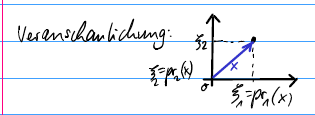
\includegraphics[width=5cm,height=3cm]{Veranschaulichung}
	\end{figure}\\
	\underline{Bem.:}$\bullet$ Die Abb. $pr_j$ ist eine Lineare Abb.\\
	$\bullet$ Bei $x_k\rightarrow a$ erspart uns die Notation $pr_j (x_k)$ die 
	benutzung von Doppelindezes "$\xi_{kj}$". Konvergenz im $\mathbb{R}^n$ gilt 
	Komponentenweise, d.h für \underline{jede} Koordinate einzeln:\\
	\textbf{1.12\underline{Bem.:}} Im $\mathbb{R}^n$ gilt: 
	\setulcolor{green}\ul{$x_k 
	\xrightarrow{k\rightarrow \infty} a \Leftrightarrow \forall_j \in 
	{1,...,n}: pr_j(x_k)\rightarrow pr_j(a)$}.\\
	\underline{Bew.:} Für j steht fest und alle k ist $|pr_j(x_k) - pr_j(a)| 
	\leq ||x_k-a||_\infty$,\\
	was "$\Rightarrow$" zeigt. Wegen $||x_k-a||_\infty = \underset{1\leq j \leq 
	n}{\max}{pr_j (x_k)-pr_j(a)}$ folgt "$\Leftarrow$".\hfill$\square$\\
	\\
	\textbf{1.13. \underline{Bem.:}} Aus der Linearen Algebra I/II ist bekannt 
	(vgl Anhang Nr.6.), dass es neben dem (euklidischen) Standardskalarprodukt 
	noch mehr Skalarprodukte $\textless,\textgreater$ gibt, die dann gemäß der 
	Setzung $||x||:=\textless x,x\textgreater$ noch andere Normen induzieren, 
	Ob und wie sich das auswirkt, untersuchen wir in Teil 2 Dieser Vorlesung, 
	wo wir allgemeinr normierte Vektorräume und Metrische Räume zulassen und 
	deren Analysis erarbeiten werden. In diesen teil 1 beschränken wir uns 
	zunächst auf den Fall $\mathbb{R}^n$, in Teil 2 wird also der "höhere 
	Standpunkt" untersucht. Teil 3 der Vorlesung behandelt dann gewöhnliche 
	Differentialgleichungen.
\end{document} 
